\documentclass[10pt, twocolumn, a4j, platex]{jsarticle}	% Japanese
\usepackage[subrefformat=parens]{subcaption}
\usepackage{enumerate}
\usepackage{booktabs}
\usepackage[dvipdfmx]{graphicx}
\usepackage[dvipdfmx]{color}
\usepackage{amsmath}
\usepackage[varg]{txfonts}
\usepackage{comment}
\usepackage{float}
\usepackage{threeparttable}
\usepackage{caption}
\usepackage{etoolbox}
\usepackage{vtable,hhline}
\usepackage{siunitx}
\AtBeginEnvironment{table}{\captionsetup{justification=centering}}
\bibliographystyle{IEEEtran}
\pagestyle{empty} %ページ番号非表示
\renewcommand{\baselinestretch}{0.68}	%ストレッチ
\renewcommand{\rmdefault}{ptm}			%Timesフォント
\setlength{\textwidth}{186mm}			%本文全幅    210-1inch(25.4)*2-186+13.4*2 = 0
\setlength{\textheight}{276.2mm}		%本文全高    297-1inch(25.4)*2-276.2+15*2 = 0
\setlength{\oddsidemargin}{-13.4mm}		%用紙左余白  210-1inch(25.4)*2-186+13.4*2 = 0
\setlength{\evensidemargin}{-13.4mm}	%用紙左余白  210-1inch(25.4)*2-186+13.4*2 = 0
\setlength{\topmargin}{-15mm}			%用紙上の余白 297-1inch(25.4)*2-276.2+15*2 = 0
\setlength{\headheight}{0mm}			%ヘッダーの高さ
\setlength{\headsep}{0mm}			    %ヘッダーと本文までの高さ
\setlength{\footskip}{0mm}			    %フッターと本文の高さ
\setlength{\textfloatsep}{3mm}			%本文と図の間のスペース
% \usepackage[acronym,shortcuts]{glossaries} % disabled: causes UTF-8 regex error under pLaTeX (datatool-utf8)
\setlength\intextsep{1pt}
\setlength\textfloatsep{8pt}
\usepackage{url}
\newcommand{\argmax}{\mathop{\rm arg~max}\limits}
\newcommand{\argmin}{\mathop{\rm arg~min}\limits}
% 参照系
\newcommand{\wpage}[1]{\pageref{#1}ページ}%
\newcommand{\weq}[1]{式(\ref{eq:#1})}%
\newcommand{\wfig}[1]{図\ref{fig:#1}}%
\newcommand{\wtab}[1]{表\ref{tab:#1}}%
\newcommand{\wpro}[1]{プログラム\ref{pro:#1}}%
\newcommand{\wsec}[1]{\ref{sec:#1}}%
\newcommand{\wpeq}[1]{\wpage{eq:#1}\weq{#1}}%
\newcommand{\wpfig}[1]{\wpage{fig:#1}\wfig{#1}}%
\newcommand{\wptab}[1]{\wpage{tab:#1}\wtab{#1}}%
\newcommand{\wppro}[1]{\wpage{pro:#1}\wpro{#1}}%
\newcommand{\wpsec}[1]{\wpage{sec:#1}\wsec{#1}}%
\newcommand{\wsubfig}[2]{\wfig{#1}\subref{fig:#2}}%\wsubfig{caption}{subcaption}
\begin{document}
\makeatletter
\def\section{\@startsection {section}{1}{\z@}{3 ex}{1ex}{\large\bf}}
\def\subsection{\@startsection {subsection}{1}{\z@}{3ex}{1ex}{\normalsize\bf}}
\def\subsubsection{\@startsection {subsubsection}{1}{\z@}{1ex}{1ex}{\normalsize\bf}}
\makeatother
% --------------------------------------------------------------------- %
\twocolumn[
	\begin{center}
		% header
		{\small 2024年度 電気通信大学 情報理工学域$\mathrm{I}\hspace{-1.2pt}\mathrm{I}$類 情報通信工学プログラム 卒業研究中間発表会 AWCC藤井研究室予稿}\\
		\vspace{1zw}
		% title
		{\bf \Large V2X・ドローン向けマルチバンド連携による通信安定化手法の研究}\\
		\vspace{1zw}
		%author
		{\small 発表者 : 2210177 鐘ヶ江僚太, 指導教員 :  藤井威生 教授}\\
		{\small 先端ワイヤレス・コミュニケーション研究センター(AWCC) 藤井研究室}
		% % 連絡先
		% \\ \vspace{1zw}
		% \normalsize{\itshape{
		% 		Advanced Wireless and Communications research Center (AWCC) \\
		% 		The University of Electro-Communications \\
		% 		1-5-1 Chofugaoka, Chofu, Tokyo, 182-8585 Japan \\
		% 		TEL:042-443-5917, FAX:042-443-5860 \\
		% 		kanegae@awcc.uec.ac.jp
		% 	}}
		\vspace{1zw}
	\end{center}
]
\section{はじめに}

第5世代移動通信システム(5G)の普及に伴い,社会のあらゆる場面で無線通信の活用が進んでいる.その一方で,研究開発の最前線はすでに2030年代の実用化を目指す「Beyond 5G」あるいは「6G」へと移行しており,テラヘルツ波の利用による超高速・大容量通信,リアルとサイバー空間を高度に融合させるサイバーフィジカルシステム(CPS)の実現などのビジョンが掲げられている.これらの次世代移動通信システムが支える重要なユースケースとして,車両が周辺の車両や交通インフラ,歩行者などと直接通信を行うV2X(Vehicle-to-Everything)通信や,自律飛行による物流・測量・警備などを実現するドローン通信が挙げられる.

これらのアプリケーション,特に高度な自動運転やドローンの見通し外運用においては,高速通信と同時に,途切れることのない高信頼な通信が必要となる.この要求を満たすため,広帯域を確保可能なミリ波の活用が不可欠とされているが,ミリ波は物理的な遮蔽に対して脆弱であり,高速移動するV2Xやドローン通信環境では,通信の瞬断が頻発するという根本的な課題を抱えている.このミリ波の遮蔽に対する脆弱性は,安全性や信頼性が最優先されるアプリケーションの実用化における深刻なボトルネックとなっている.

この課題に対し,ミリ波とより安定したSub-6GHz帯などを連携させるマルチバンド通信が有効な解決策として研究されている.従来のアプローチの多くは,受信信号強度(RSSI)や信号対干渉雑音比(SINR)といった通信品質の劣化を観測した後に,より安定した周波数帯への切り替えを行う事後対応的な制御が中心であった.この手法はシンプルで有効な場面も多いが,品質劣化の検知から切替完了までの間に避けられない遅延が生じ,その間の通信断を完全に防ぐことは困難である.

一方で,V2Xやドローンの移動軌跡がある程度予測可能である特性を利用し,遮蔽発生を事前に予測して事前対応的にバンド切り替えを行う研究も進められている.しかし,予測のみに依存する手法は,予測誤差による不要な切り替えを引き起こす可能性や,予測不可能な突発的な通信環境の変化に対応できないという脆弱性を持つ.

そこで本研究では,これら両アプローチの長所を統合することを目指す.具体的には,通信環境が良好な場合にはミリ波を主回線として使用し,遮蔽が予測される場合にはSub-6GHz帯を補助的に活用するハイブリッド制御を提案する.このハイブリッド制御を実現するため,2つの具体的な手法を検討する.第一に,予期しない通信エラーが発生した場合や,予測される遮蔽が短時間である場合に,ミリ波での通信を維持しつつ,失敗したパケットのみを低周波数帯で迅速に再送するリカバリ手法を検討する.第二に,長時間の遮蔽が予測される場合や,観測される通信品質が継続して閾値を下回った場合に,通信が途絶する前に低周波数帯への能動的なバンド切り替え手法を検討する.

\section{既存研究}

事後対応的な制御は,通信品質の劣化を観測した後に制御を行うアプローチである.RSSIやSINRなどの指標を監視し,その値が閾値を下回った場合に,より安定した周波数帯へ通信を切り替える.Perfectoら\cite{0001}は,隊列走行を対象とし,主回線であるミリ波リンクが切断された際に,Sub-6GHz帯のバックアップリンクで通信を補完する手法を提案した.また,Gapeyenkoら\cite{0002}は,ミリ波とSub-6GHz帯への同時接続によるデュアルコネクティビティの実現可能性を評価し,チャネル品質に基づいて動的に通信経路を選択することで接続信頼性を向上させる手法を検討している.これらの手法は,予測不能な通信環境の変化に対応できる利点を持つが,品質劣化の検知から切り替え完了までの間に遅延が生じるという課題がある.

事前対応的な制御は,移動体の軌跡や周辺環境情報を用いて通信品質の劣化を事前に予測し,通信が不安定になる前に制御を行うアプローチである.車両やドローンの移動の予測可能性を活用する点が特徴である.Vaら\cite{0003}は,車両の位置と速度から将来位置を予測し,路側帯基地局との間で最適となるミリ波ビームを事前に選択・切り替えする手法を提案した.これにより,通信リンクが途切れる前にビームを追従させ,通信の継続性を高めている.ドローンを対象とした研究では,Aliら\cite{0004}がドローンの移動パターンを予測し,サービス提供基地局を事前に切り替えるプロアクティブ・ハンドオーバを提案している.このアプローチは,理論上,通信の瞬断を未然に防ぐことが可能だが,予測精度に性能が大きく依存する.

ハイブリッドアプローチとして,Kimら\cite{0005}は,車両の走行コンテキスト(交差点,直進など)を認識し,状況に応じて事前対応的な制御と事後対応的な制御を使い分ける手法を検討している.また,Palaciosら\cite{0006}は,LiDARセンサーによる前方遮蔽物の検知に基づく事前対応的なバンド切り替えを基本としつつ,予測が失敗した場合や突発的な遮蔽が発生した際には,リアクティブな品質監視に基づく切り替えで補完するハイブリッド手法を提案した.これらの研究は,予測と実測情報を組み合わせることで,より頑健な通信の実現を目指している.

\section{提案手法}

本研究の目的は,V2Xおよびドローン通信におけるミリ波の遮蔽問題を解決するため,マルチバンド連携による通信安定化手法を提案・評価することである.具体的には,ミリ波とSub-6GHz帯を組み合わせたハイブリッド制御を実現し,通信の信頼性と効率性を両立させることを目指す.

本研究では,以下の2つの主要な手法を検討する.1つ目は選択的リカバリ手法である.予期しない通信エラーが発生した場合や,予測される遮蔽が短時間である場合に,ミリ波での通信を維持しつつ,失敗したパケットのみを低周波数帯で迅速に再送する手法である.この手法により,ミリ波の高帯域幅を活かしつつ,通信の信頼性を向上させることが可能となる.2つ目は能動的にバンドを切り替える手法である.長時間の遮蔽が予測される場合や,観測される通信品質が継続して閾値を下回った場合に,通信が途絶する前に低周波数帯へ切り替える手法である.

これらの手法を組み合わせることで,通信の安定性を保ちつつ,ミリ波による高速通信の利点を最大限に活用することを目指す.

\section{初期検討}

\begin{figure}[tb]
	\centering
	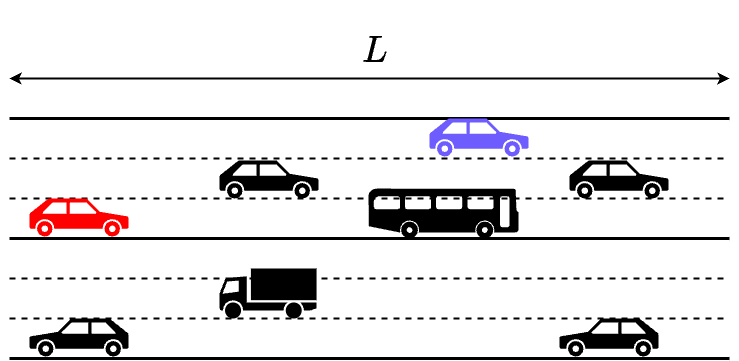
\includegraphics[width=0.95\linewidth]{./images/model.drawio.png}
	\caption{シミュレーションモデル} \label{fig:model}
\end{figure}

初期検討として,同一通信環境において,ミリ波通信とSub-6GHz帯通信のSINRとスループットを比較した.本稿では\wfig{model}に示すように片側3車線の直線道路を想定し,遮蔽物として一般車両だけでなく,バスやトラックなどの大型車両も存在する環境にてシミュレーションを行った.これらの車両はランダムに車線変更を行い,実際の交通状況を模擬した.送受信車両はそれぞれ1台ずつとした.

\subsection{SINRとスループットの測定}

今回のシミュレーションにおいて,SINRとスループットを直接測定するために以下の計算式を用いた.

\begin{equation}
	\mathrm{SINR} = \frac{P_{\mathrm{s}}}{P_{\mathrm{i}} + P_{\mathrm{n}}}
\end{equation}

\begin{equation}
	\mathrm{Throughput} = \frac{N_{\mathrm{Rx}}}{T}
\end{equation}

ここで,$P_{\mathrm{s}}$は受信信号の電力,$P_{\mathrm{i}}$は干渉信号の電力,$P_{\mathrm{n}}$は受信機のノイズ電力を表し,$N_{\mathrm{Rx}}$は受信したデータ量[byte],$T$は測定時間[s]を表す.

チャネルモデルとして,3GPP TS 38.901 UMi Street Canyonチャネルモデルを使用し,各周波数帯におけるミリ波(28GHz帯)とSub-6GHz帯(3.5GHz帯)の2つの周波数帯を比較した.シミュレーションはSUMO,Omnet++,Veinsを用いて行った.また初期検討では,各周波数帯のSINRやスループットの遮蔽物による変化を観測するため,単一の周波数帯で通信を行い,マルチバンド連携は行わなかった.今回のシミュレーション諸元を\wtab{params}に示す.

\begin{table}[tb]
	\centering
	\caption{シミュレーション諸元}
	\begin{tabular}{c|c}
		\hline
		パラメータ      & 値                   \\
		\hline
		シミュレーション時間 & \SI{60}{s}          \\
		道路長 $L$    & \SI{2}{km}          \\
		車線幅        & \SI{3.5}{m}         \\
		車線数        & 3                   \\
		初期送受信車両間距離 & \SI{50}{m}          \\
		送受信車両速度    & \SI{60}{km/h}       \\
		一般車両数      & 35台                 \\
		大型車両数      & 8台                  \\
		一般車両速度     & 40 -- \SI{60}{km/h} \\
		大型車両速度     & 40 -- \SI{50}{km/h} \\
		28GHz帯域幅   & \SI{100}{MHz}       \\
		3.5GHz帯域幅  & \SI{20}{MHz}        \\
		\hline
	\end{tabular}
	\label{tab:params}
\end{table}

\subsection{シミュレーション結果}

シミュレーションの結果,得られたSINRとスループットをそれぞれ\wfig{sinr}と\wfig{throughput}に示す.このように,ミリ波はSub-6GHz帯に比べてSINRが大きく変動し,遮蔽物による影響を強く受けることが分かる.またスループットに関しても,ミリ波はSub-6GHz帯に比べて高い値を示す一方で,遮蔽物の影響で大きく低下することが確認できた.これらの結果から,ミリ波通信は高速通信が可能である一方で,遮蔽物による通信品質の劣化が顕著であることが分かり,マルチバンド連携による通信安定化手法の必要性が示唆された.

\begin{figure}[tb]
	\centering
	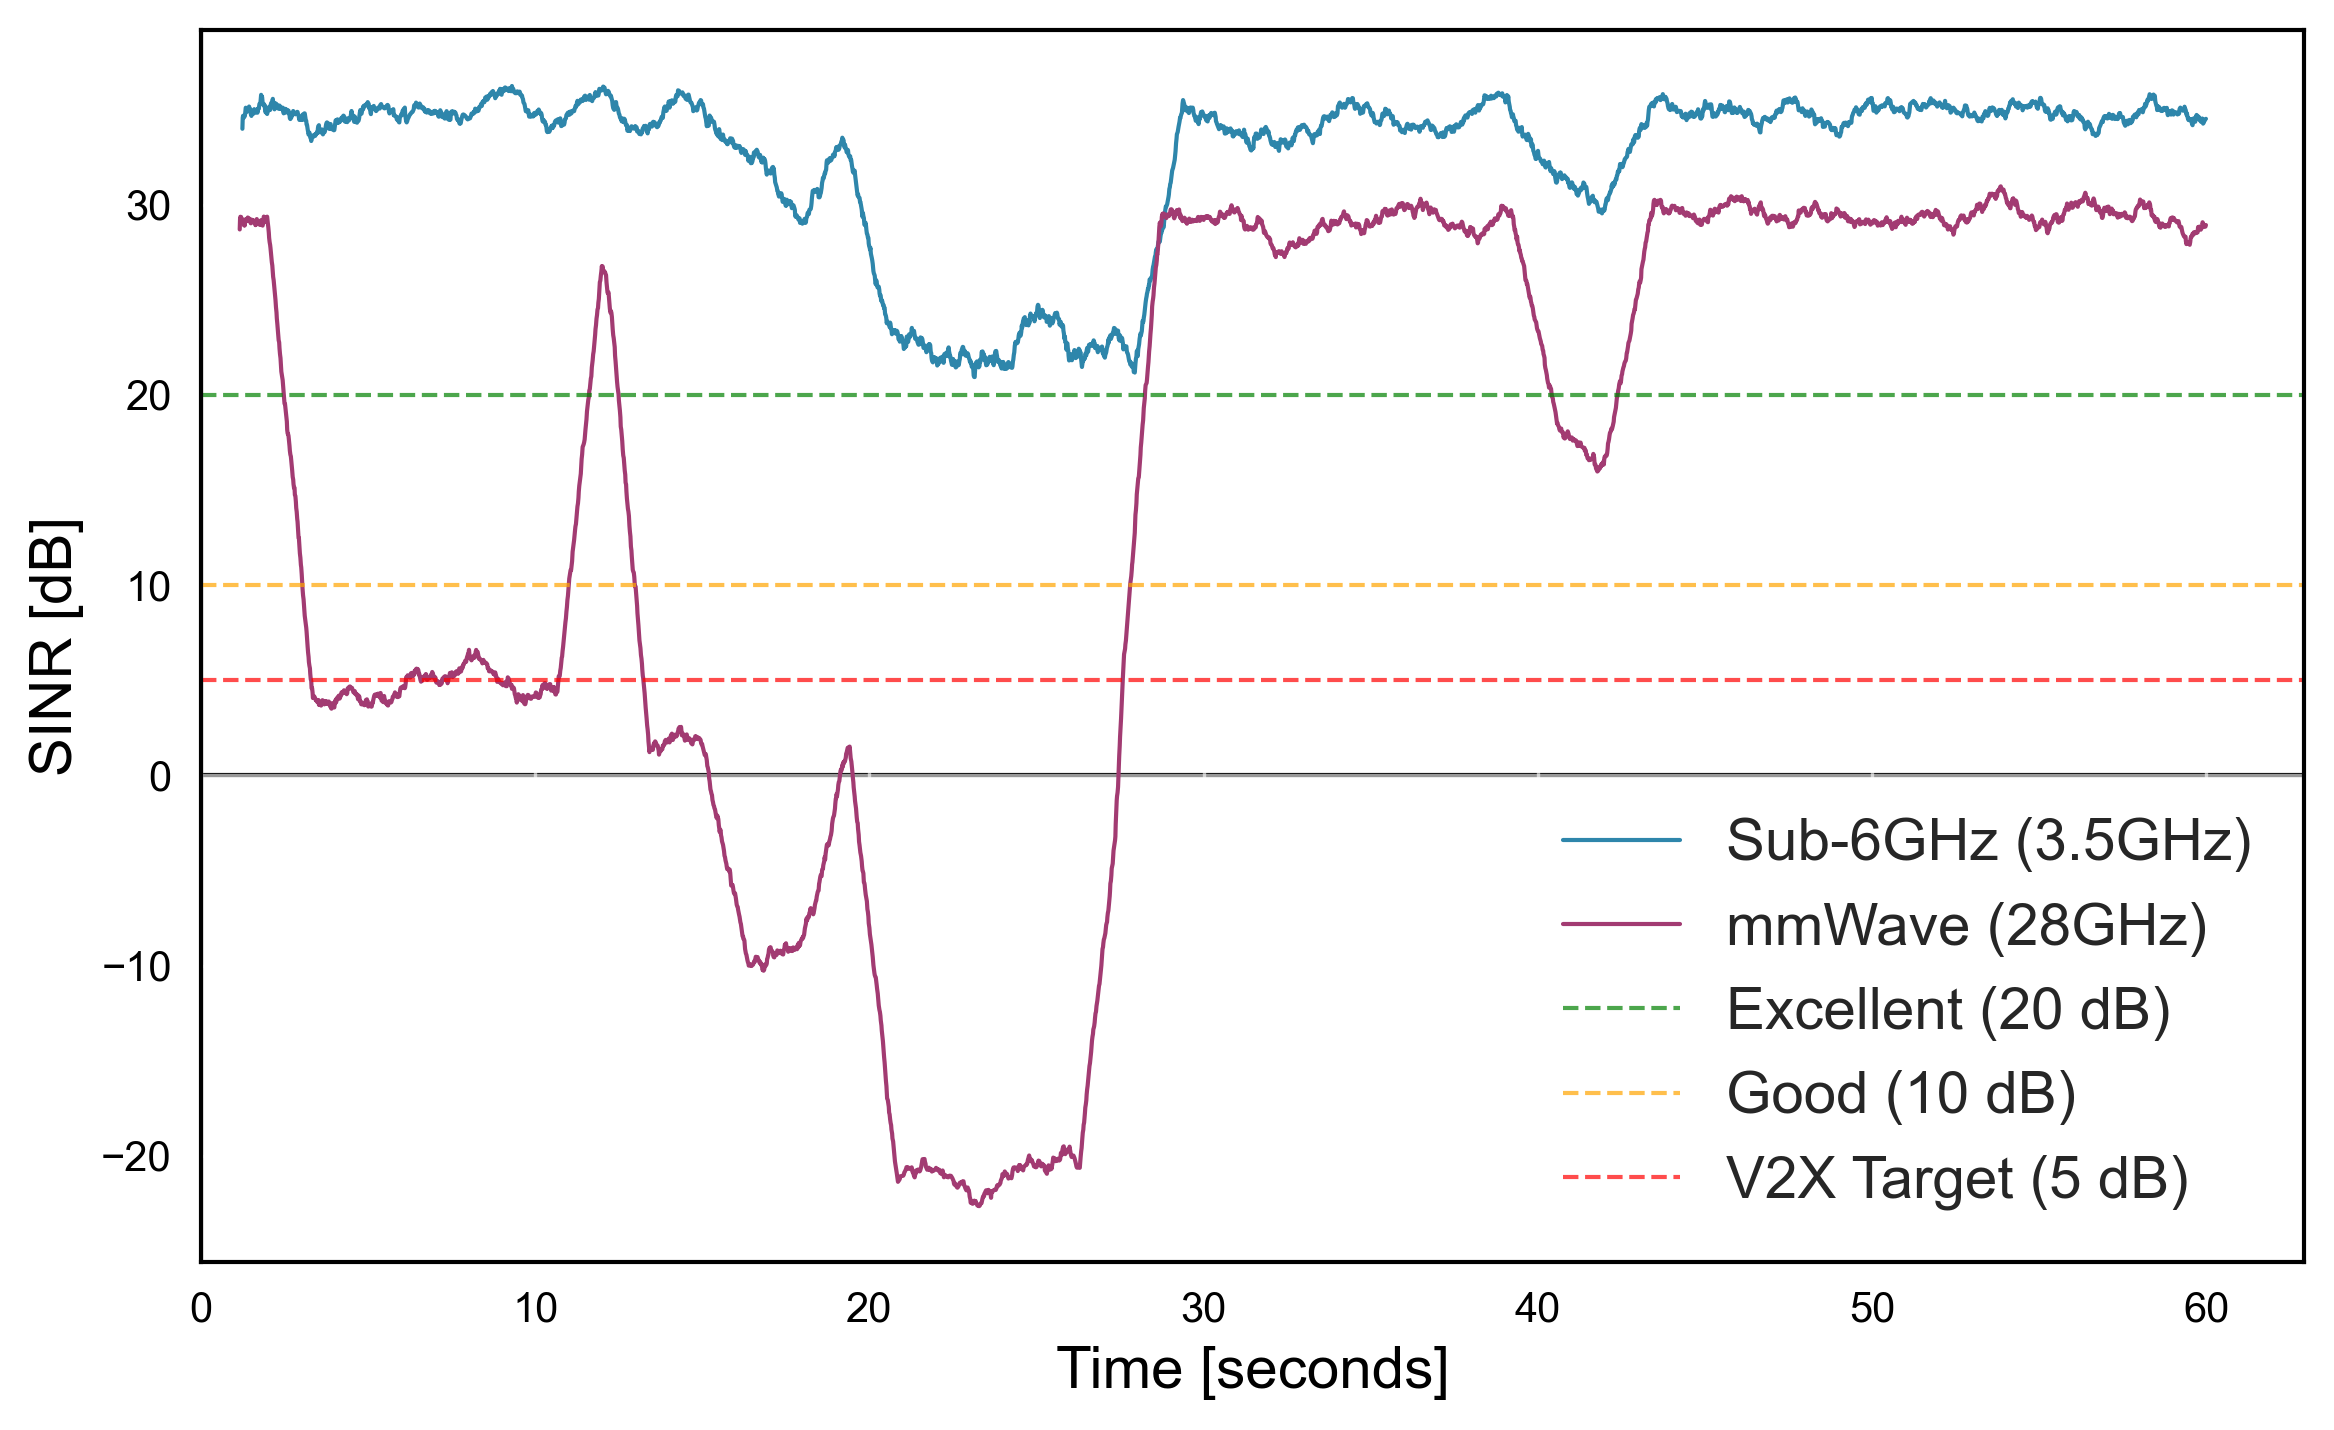
\includegraphics[width=0.95\linewidth]{./images/sinr_comprehensive_analysis.png}
	\caption{各周波数帯のSINR} \label{fig:sinr}
\end{figure}

\begin{figure}[tb]
	\centering
	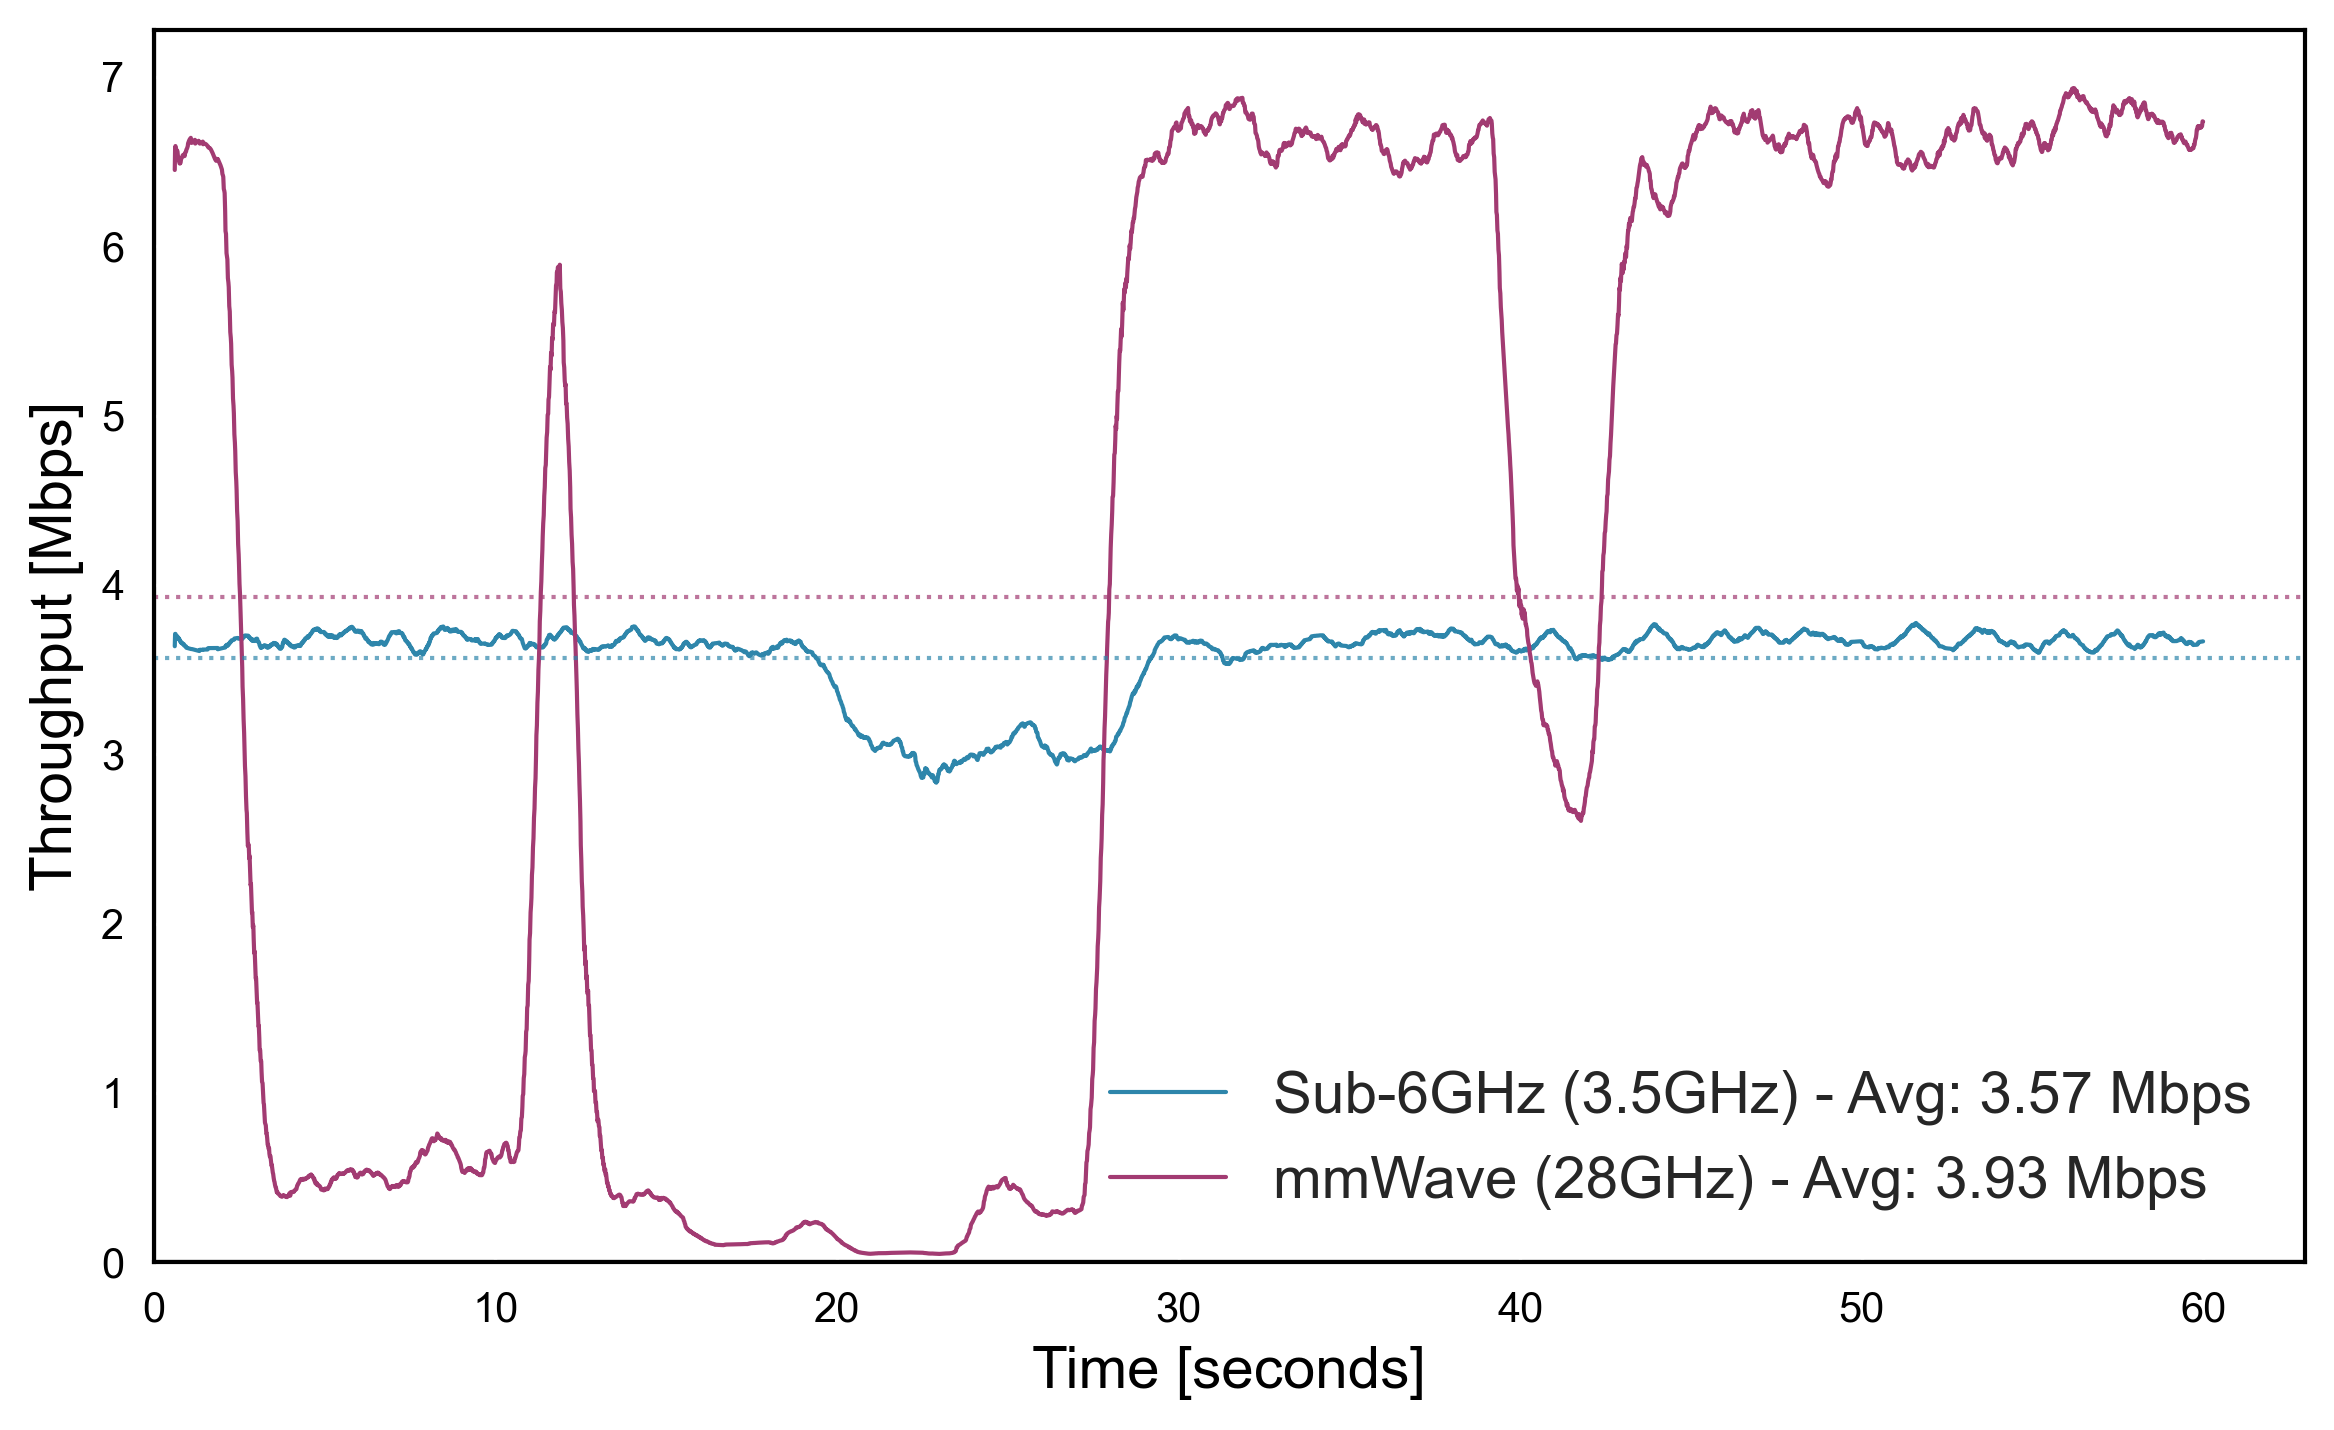
\includegraphics[width=0.95\linewidth]{./images/harq_comprehensive_analysis.png}
	\caption{各周波数帯のスループット} \label{fig:throughput}
\end{figure}

\section{まとめと今後の研究方針}

本稿では,V2Xおよびドローン通信におけるミリ波の遮蔽問題を解決するため,マルチバンド連携による通信安定化手法を提案・評価することを目的とした.初期検討として,同一通信環境においてミリ波通信とSub-6GHz帯通信のSINRとスループットを比較し,ミリ波が高速通信を可能にする一方で,遮蔽物による通信品質の劣化が顕著であることを確認した.これらの結果から,マルチバンド連携による通信安定化手法の必要性が示唆された.

今後の研究では,提案するハイブリッド制御手法の具体的なアルゴリズム設計とシミュレーション評価を進める.まず,予期しない通信エラーが発生した場合や,予測される遮蔽が短時間である場合に,ミリ波での通信を維持しつつ,失敗したパケットのみを低周波数帯で迅速に再送する選択的リカバリ手法を詳細に検討する.次に,長時間の遮蔽が予測される場合や,観測される通信品質が継続して閾値を下回った場合に,通信が途絶する前に低周波数帯への能動的なバンド切り替え手法を設計する.これらの手法を組み合わせたハイブリッド制御アルゴリズムを実装し,シミュレーション環境でその性能を評価する.さらに,実際のV2Xおよびドローン通信環境での実験も視野に入れ,提案手法の実用性と効果を検証する予定である.

\bibliography{main}

\end{document}
